\begin{tabular}[b]{c}
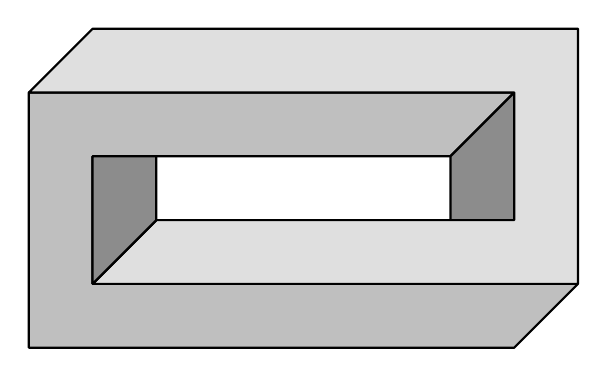
\begin{tikzpicture}[scale=4.5, line join=bevel]
  % \a and \b are two macros defining characteristic
  % dimensions of the impossible brick.
  \pgfmathsetmacro{\a}{0.18}
  \pgfmathsetmacro{\b}{1.37}
  \tikzset{%
    apply style/.code={\tikzset{#1}},
    brick_edges/.style={thick,draw=black},
    face_colourA/.style={fill=gray!50},
    face_colourB/.style={fill=gray!25},
    face_colourC/.style={fill=gray!90},
  }
  \foreach \theta/\v/\facestyleone/\facestyletwo in {%
    0/0/{brick_edges,face_colourA}/{brick_edges,face_colourC},
    180/-\a/{brick_edges,face_colourB}/{brick_edges,face_colourC}
  }{
  \begin{scope}[rotate=\theta,shift={(\v,0)}]
    \draw[apply style/.expand once=\facestyleone]  		
      ({-.5*\b},{1.5*\a}) --
      ++(\b,0)            --
      ++(-\a,-\a)         --
      ++({-\b+2*\a},0)    --
      ++(0,-{2*\a})       --
      ++(\b,0)            --
      ++(-\a,-\a)         --
      ++(-\b,0)           --
      cycle;
    \draw[apply style/.expand once=\facestyletwo] 
      ({.5*\b},{1.5*\a})  --
      ++(0,{-2*\a})       --
      ++(-\a,0)           --
      ++(0,\a)            --
      cycle;
    \end{scope}
  }
\end{tikzpicture}\\
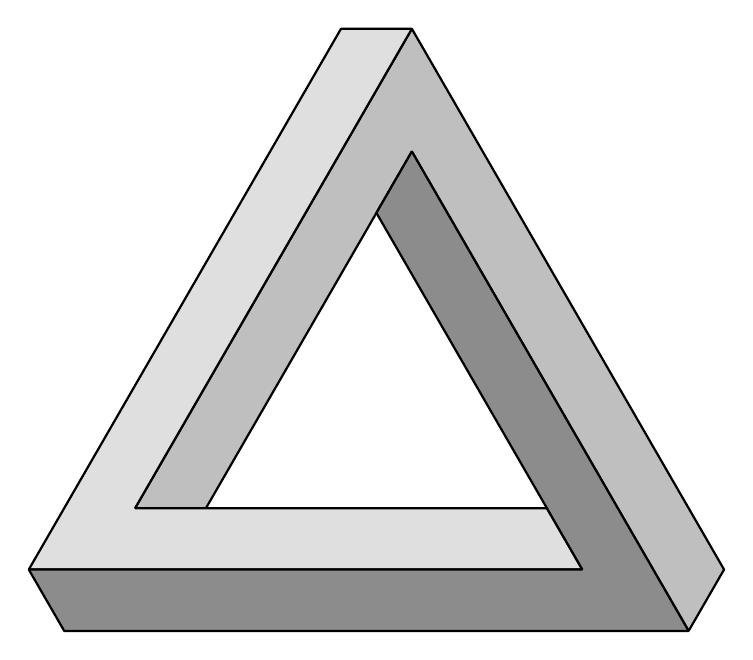
\begin{tikzpicture}[scale=1, line join=bevel]
% \a and \b are two macros defining characteristic
% dimensions of the Penrose triangle.		
\pgfmathsetmacro{\a}{2.5}
\pgfmathsetmacro{\b}{0.9}
\tikzset{%
  apply style/.code     = {\tikzset{#1}},
  triangle_edges/.style = {thick,draw=black}
}
\foreach \theta/\facestyle in {%
    0/{triangle_edges, fill = gray!50},
  120/{triangle_edges, fill = gray!25},
  240/{triangle_edges, fill = gray!90}%
}{
  \begin{scope}[rotate=\theta]
    \draw[apply style/.expand once=\facestyle]
      ({-sqrt(3)/2*\a},{-0.5*\a})                     --
      ++(-\b,0)                                       --
        ({0.5*\b},{\a+3*sqrt(3)/2*\b})                -- % higher point	
        ({sqrt(3)/2*\a+2.5*\b},{-.5*\a-sqrt(3)/2*\b}) -- % rightmost point
      ++({-.5*\b},-{sqrt(3)/2*\b})                    -- % lower point
        ({0.5*\b},{\a+sqrt(3)/2*\b})                  --
      cycle;
    \end{scope}
  }	
\end{tikzpicture}%
\end{tabular}%
